\chapter{Cryptography techniques}
Cryptography is a mathematical technique that permits to transmit the data to a form that can't be understood by unauthorized users.
\begin{figure}[H]
    \centering
    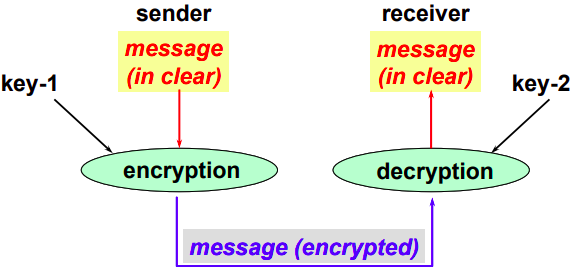
\includegraphics[width=0.5\textwidth]{/home/lorenzo/Notes/Information System Security/images/image copy 13.png}
\end{figure}
\noindent
To explain the various concepts of cryptography we need to introduce some terminology:
\begin{itemize}
    \item \textbf{Plaintext (P)}: the original message before encryption.
    \item \textbf{Ciphertext (C)}: the encrypted message that appears scrambled.
\end{itemize}
\begin{quotebox-grey}{Kerckhoffs' Principle}
\begin{minipage}{0.7\textwidth}
	\vspace{-0.3cm}
This principle states that the security of a cryptographic system should rely on the \textbf{secrecy of the keys}, not the secrecy of the encryption algorithm itself. 
If the keys:
\begin{itemize}
\item are kept secure, this ensures only authorized parties can decrypt the message.
\item are managed by trusted systems, this minimizes the risk of unauthorized access.
\item are of adequate length, they are harder to crack with brute force methods. 
\end{itemize} 
\end{minipage} 
\hspace{0.3cm}
\begin{minipage}{0.3\textwidth}
    \centering
    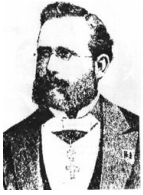
\includegraphics[width=0.4\textwidth]{/home/lorenzo/Notes/Information System Security/images/image copy 14.png}
\end{minipage}
\noindent
\\
\\
\textbf{It's no important that the encryption and decryption algorithms are kept secret}, on the contrary it's better to make the algorithms public so that they can be widely analysed and their possible weakness identified. 
\\
\\
Kerchoff’s Principle is tightly correlated to the principle of \textbf{Security Through Obscurity
(STO)}: a system is protected but the details on how it has been protected are not disclosed.
This alone is not considered a valid security mechanism. STO can be used as a layer of the security system \textbf{only if} a really strong algorithm is used
\end{quotebox-grey}
\newpage
\section{Symmetric Cryptography}
\textbf{Symmetric cryptography} is so called because it uses \textbf{only} a single key \textbf{shared between} the sender and the receiver. 
\[key1=key2=K\]
The key \textbf{K} is used to generate the Ciphertext \textbf{C} by encrypting the Plaintext \textbf{P}. \textbf{C} is then sent to the receiver, which recovers \textbf{P} by applying the decryption algorithm using \textbf{K}:
\[C\ =\ enc(K,P)\ =\ \{P\}K\]
\[P\ =\ dec(K,C)\ =\ enc^{-1}(K,C)\]
\begin{figure}[H]
    \centering
    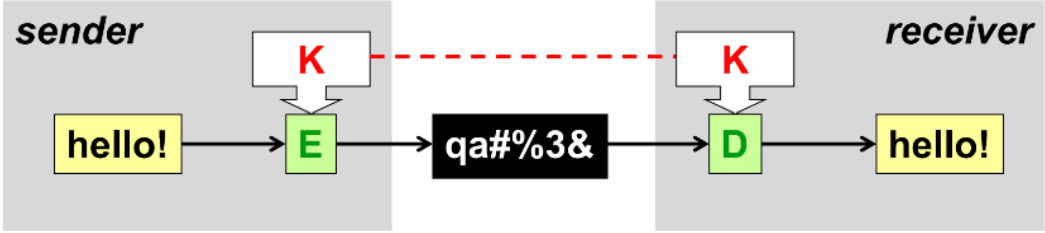
\includegraphics[width=0.5\textwidth]{/home/lorenzo/Notes/Information System Security/images/Screenshot from 2024-12-27 13-04-27.png}
\end{figure}
\noindent
\textbf{Symmetric Encryption} requires the use of a unique \textbf{K} for each peer couple. A complete pairwise private communication between N parties would requires:
 \[\frac{N \cdot (N-1)}{2}\ \text{unique \textbf{K}s}\]
The parties can exchanged \textbf{securely} the \textbf{K}s in two ways:
\begin{itemize}
    \item \textbf{OOB} (\textbf{Out-Of-Band}): the parties share the \textbf{K} without using electronic channel used for transmitting the encrypted message.
    \item \textbf{Key Exchange Algorithms}: algorithms such as Diffie-Helmann enable parties to securely exchange keys over a potentially insecure channel.
    \begin{figure}[H]
        \centering
        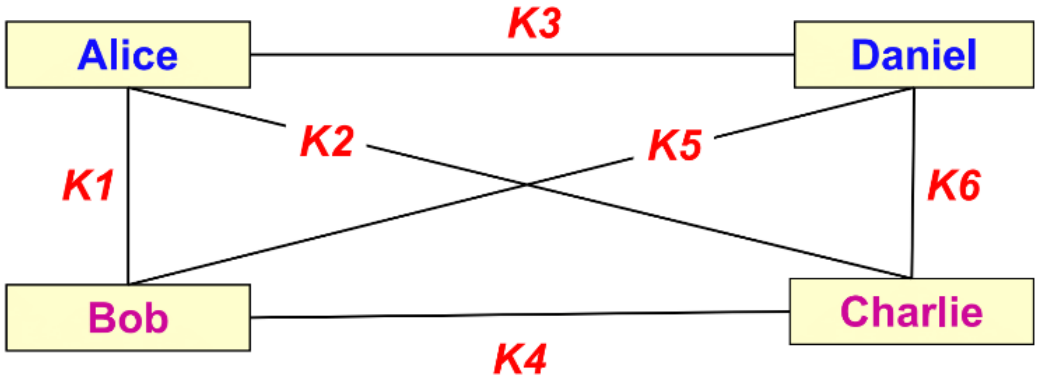
\includegraphics[width=0.4\textwidth]{/home/lorenzo/Notes/Information System Security/images/Screenshot from 2024-12-27 15-26-15.png}
    \end{figure}   
\end{itemize}
\begin{quotebox-grey}{Symmetric Block Encryption Algorithms}
    The main type of symmetric is the \textbf{Block Algorithm}. Each algorithm elaborates encryption/decryption \textbf{only if} a minimum amount of data  (typically 64/128 bits) is available.
    \vspace{0.2cm}
        \begin{center}
            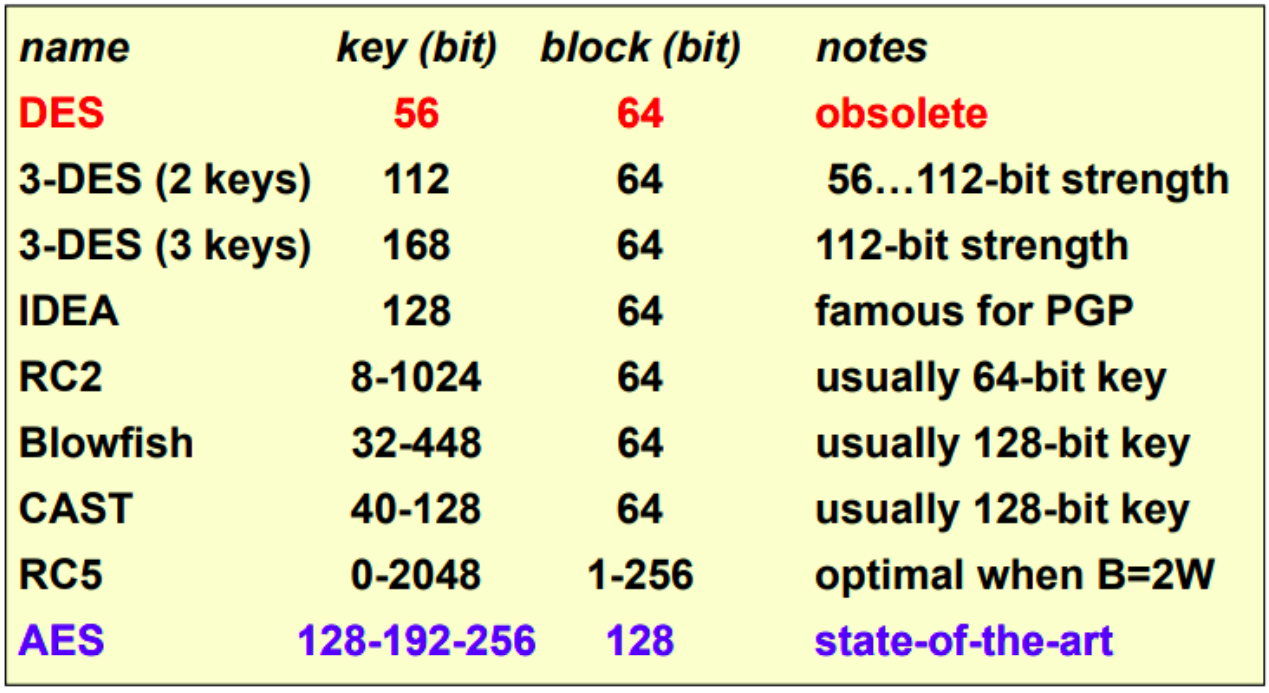
\includegraphics[width=0.5\textwidth]{/home/lorenzo/Notes/Information System Security/images/Screenshot from 2024-12-27 15-57-24.png}
        \end{center}
\end{quotebox-grey}

\newpage
\subsection{DES (Data Encryption Standard)}
DES uses \textbf{64 bits keys}, yet its effectiveness is only the one of a 56 bits key, since 8 bits of the key are used to check the parity of the others. This means that, when DES generates a key, every 7 bits that are generated, another is added to check the parity of the previous 7 bits. It's designed to be \textbf{efficient in hardware} because it requires: 
\begin{itemize}
    \item \textbf{XOR in details}: elementary operation on all the CPUs.
    \begin{quotebox}[colframe=blue!10!white, colback=blue!5!white]{XOR}
        It's a fundamental operation in cryptography, it provides "confusion" by randomizing input data.
        ruth table:
        \begin{center}
        \begin{tabular}{|c|c|c|}

\hline
A & B & A XOR B \\
\hline
0 & 0 & 0 \\
0 & 1 & 1 \\
1 & 0 & 1 \\
1 & 1 & 0 \\
\hline
\end{tabular}
\end{center}

Notes that it's the \textbf{inverse of itself}:
\begin{itemize}
    \item if \(A\ xor\ B\ =\ Z\) then \(Z\ xor\ B\ =\ A\) (or \(Z\ xor\ A\ =\ B\))
\end{itemize}
    \end{quotebox}
    \item \textbf{Shift}: elementary operation on all the CPUs.
    \item \textbf{Permutation}: expensive operation  yet efficient if done directly in hardware.
    \begin{figure}[H]
        \centering
        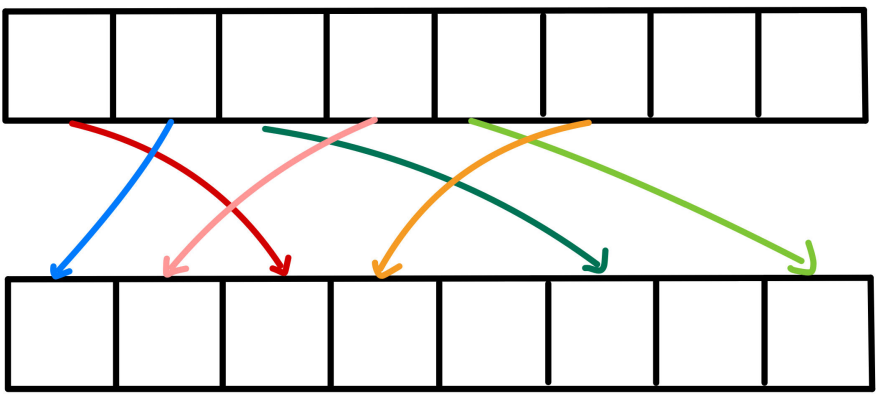
\includegraphics[width=0.3\textwidth]{/home/lorenzo/Notes/Information System Security/images/Screenshot from 2024-12-27 15-56-26.png}
    \end{figure}
\end{itemize}

\subsection{3-DES or Triple DES}
It was introduced as an improved version of the original DES. It is simply the repeated application of the DES. It uses \textbf{two} or \textbf{tree} keys. Usually, 3-DES is applied in the \textbf{EDE} (\textbf{Encryption-Decryption-Encryption}) \textbf{mode}:
\begin{itemize}
    \item \textbf{With 2 keys} \(\rightarrow \) Uses two 56-bit keys (K1 and K2), repeating K1 for the
    third operation:
    \[C'\ =\ enc(K_1,P)\ \ \ C''=dec(K_2,C')\ \ \ C=enc(K_1,C'')\]
    \begin{quotebox-red}{Beware}
        If sufficient memory is available for attack (about \(2^{59} B\)), the effective security
        of this scheme is roughly \textbf{56 bits}, due to vulnerabilities. Without that much
        memory, the effective key size is \textbf{12 bits}.
    \end{quotebox-red}
    \item \textbf{With 3 keys} \(\rightarrow \) Uses three distinct keys (K1, K2, and K3), providing better security with an effective key size of 112 bits:
    \[C'\ =\ enc(K_1,P)\ \ \ C''=dec(K_2,C')\ \ \ C=enc(K_3,C'')\]
\end{itemize}
\begin{customquote}
\vspace{-0.4cm}
\subsubsection{Why 2-DES is not used?}
Because the double application of any encryption algorithm is subject to a \textbf{Known-Plaintext Attack}, which is a kind of MIMT attack. This attack allows to decrypt data with \textbf{at most \(2^{N+1}\)} attempts (if the keys are N-bit long).
\\
\\
During a Known-Plaintext attack both \textbf{P} and \textbf{C} (\(=enc(K_2,enc(K_1,P))\) are \textbf{sniffed by} the attacker. Hypothesizing N bits keys, the attacker can then compute \textbf{K} by:
\begin{enumerate}
    \item Compute \(2^N\) values \(X_i=enc(K_i,P)\)
    \item Compute \(2^N\) values \(Y_j=dec(K_j,C)\)
    \item Search of those values \(K_i\) and \(K_j\) such that \(X_i=Y_j\)
    \item Discard false positive
\end{enumerate}
\end{customquote}


\subsection{AES (Advanced Encryption Standard))}
AES was established through a public international competition aimed at replacing the Data Encryption Standard (DES). On October 2, 2000, Rijndael was selected as the winner of the AES competition, featuring:
\begin{itemize}
    \item Key lengths of 128, 192, or 256 bits.
    \item A block size of 128 bits.
    \item Officially published in November 2001 as FIPS-197.
    \item Gradual adoption after 2010, as cryptographic algorithms need time to prove their reliability.
\end{itemize}

\subsection{Application Modes for block algorithms}
Block algorithms are designed to encrypt \textbf{fixed-size} blocks of data, so when dealing with data of varying lengths, specific techniques must be applied:
\begin{itemize}
    \item \underline{\textbf{Size of Data to Encrypt > Algorithm's Block Size}}
    \begin{itemize}
        \item \textbf{ECB (Electronic Code Block)}: In ECB mode, each block of plaintext is encrypted independently of the others, which makes the encryption formula for the n-th block as follows:
        \[C_n=enc(K,P_n)\]
        In this mode, \textbf{decryption} is the reverse of the encryption process. The formula for decrypting the n-th block is as follows:
        \[P_n=enc^{-1}(K,C_n)\]
        Since there is no dependency between blocks, an error in transmission of one block generates an error at the decryption of only the affected block.
        \begin{figure}[H]
            \centering
            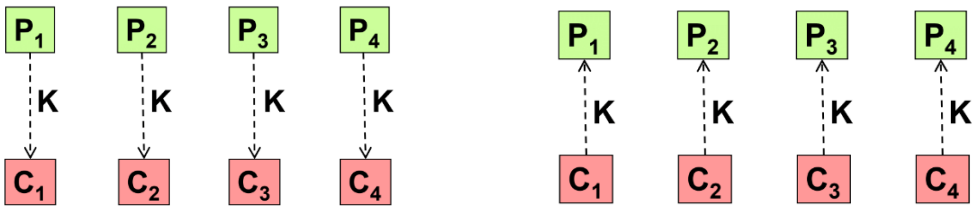
\includegraphics[width=0.7\textwidth]{/home/lorenzo/Notes/Information System Security/images/Screenshot from 2024-12-27 17-23-56.png}
        \end{figure}

        \begin{quotebox-red}{Problems with ECB mode}
            \begin{itemize}
            \item \underline{Swapping of ciphertext blocks goes undetected}: since each block is encrypted independently, if two ciphertext blocks are swapped, the decrypted message will still be valid but with blocks in the wrong order. 
            \item \underline{Identical plaintext blocks generate identical ciphertext blocks}: when two plaintext blocks are the same, their corresponding ciphertext blocks will also be identical. This lack of variation reveals patterns in the data, making it vulnerable to known-plaintext attacks 
        \end{itemize}
        \end{quotebox-red}
        \textcolor{red}{\textbf{N.B.}} \textbf{Parallel encryption and decryption are possible} because ECB blocks are independent from each other. 
        \vspace{0.1cm}
        \item \textbf{CBC (Cipher Block Chaining)}: In CBC mode, each plaintext block is XORed with the previous ciphertext block before being encrypted. The formula for encrypting the n-th block is:
        \[C_n=enc(K,P_n \oplus C_{n-1})\]
        The first plaintext block is XORed with the \textbf{IV} (\textbf{Initialization vector}) instead of a previous ciphertext block because no previous ciphertext exists for the first block. The  \textbf{IV} should be \textbf{random and unique} for every  \textbf{encryption} session.\\ 
        The \textbf{decryption} process involves reversing the encryption steps:
        \begin{figure}[h]
            \centering
            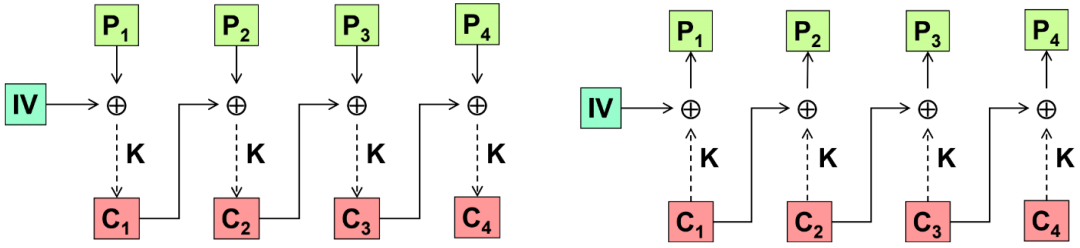
\includegraphics[width=0.8\textwidth]{/home/lorenzo/Notes/Information System Security/images/Screenshot from 2024-12-27 17-38-40.png}
        \end{figure}
        \begin{quotebox-red}{Problems with CBC mode}
            A single  error in a ciphertext block affects only two plaintext blocks:
            \begin{enumerate}
                \item The block corresponding to the erroneous ciphertext block.
                \item The next block.
            \end{enumerate}
        \end{quotebox-red}
        \textcolor{red}{\textbf{N.B.}} CBC allows for \textbf{parallel decryption} but not \textbf{parallel encryption}.
        \end{itemize}
    
    
\item \underline{\textbf{Size of data Encrypt < Algorithm's Block Size}} 
\begin{itemize}
    \item \textbf{Padding}: Padding is used to \textbf{fill the only last block} until it reaches the required block size (\textbf{C} will be longer than \textbf{P}).
    \begin{figure}[H]
        \centering
        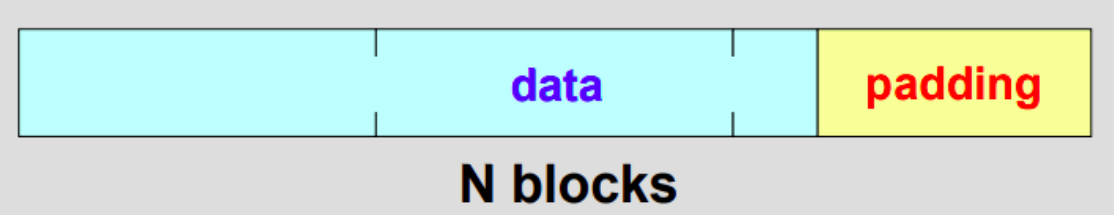
\includegraphics[width=0.5\textwidth]{/home/lorenzo/Notes/Information System Security/images/Screenshot from 2024-12-27 18-09-09.png}
    \end{figure}
    Depending on the chosen \textbf{Padding Technique}, we can allow or avoid different kind of attacks. Some techniques also offer minimal integrity control (e.g. if the key is wrong or data is manipulated, the padding bytes are incoherent).When the data size is smaller than the block size, special techniques such as \textbf{CFB} (\textbf{Cipher FeedBack}) or \textbf{OFB} (\textbf{Output FeedBack}) are the preferred.\\
    Even if the plaintext is an exact multiple of the block size, padding must still be added to avoid errors in the interpretation of the last block. 
    \vspace{0.1cm}
    \item \textbf{CTS (Ciphertext Stealing)}: CTS allows the use of block algorithms \textbf{without} the need of Padding. CTS works in the following way:
    \begin{enumerate}
        \item The last (partial block) \(P_N\) is filled with a copy of the last bytes taken from the penultimate block \(P_{N-1}\).
        \item The copied bytes are \textbf{removed} form the (now partial) penultimate block.
        \item After encryption, the last and penultimate block' positions are \textbf{exchanged}.
    \end{enumerate}
    \begin{figure}[H]
        \centering
        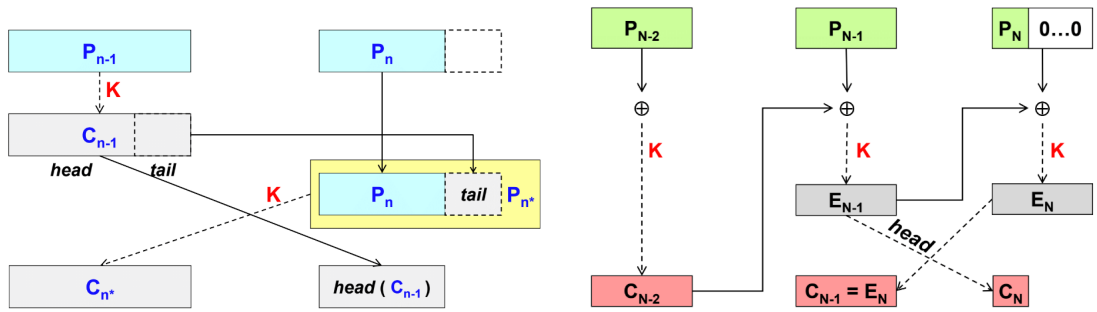
\includegraphics[width=0.7\textwidth]{/home/lorenzo/Notes/Information System Security/images/image copy 15.png}   
    \end{figure}
    \textcolor{red}{\textbf{N.B.}} CTS is particularly useful when we cannot increase the size of the data after encryption, such as in storage encryption. The computation time of encryption slightly increases due to the need for additional steps, such as modifying and swapping blocks.
    \vspace{0.1cm}
    \item \textbf{CTR (Counter Mode)}: CTR modifies block algorithm in order to encipher N bits at a time (often N = 1). CTR can be used \textbf{only} to encipher \textbf{P} smaller than one block size. It does not require padding and allows random direct access to any ciphertext block (no dependency between blocks). Requires a \textbf{nonce} and a \textbf{counter}, combined by a suitable function (concatenation, XOR, etc.) to generate the input block. CTR works in the following way:
    \begin{enumerate}
        \item \textbf{f(nonce, counter)} outputs exactly one block size of data.
        \item This block gets encrypted with the \textbf{K}.
        \item The \textbf{leftmost group} (meaning the first N bits) are extrapolated from the block and are \textbf{XOR}ed with the corresponding \(P_i\)’s group, which in turn generates the corresponding \(C_i\)’s group.
    \end{enumerate}
    \begin{figure}[H]
        \centering
        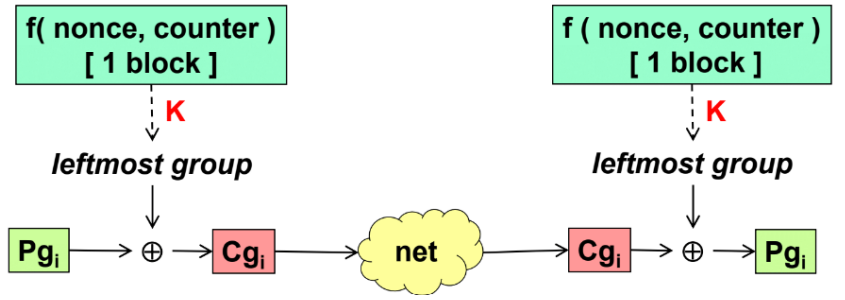
\includegraphics[width=0.7\textwidth]{/home/lorenzo/Notes/Information System Security/images/image copy 16.png}
    \end{figure}
    \begin{quotebox-red}{Cancellation attacks}
        CTR mode is vulnerable to cancellation attacks because it relies on synchronized counters between sender and receiver.    
    \end{quotebox-red}
    \begin{quotebox-yellow}{CTR as a stream ciphertext}
    The byte-oriented CTR mode of a block algorithm may be considered a stream algorithm.
    \end{quotebox-yellow}
    \textcolor{red}{\textbf{N.B.}} Moreover, if a group is \textbf{modified}, the error does not propagate to the successive group since group are independent \(\rightarrow \) it is possible to decrypt a random group \textbf{without} having decrypt the others.
    \\\textbf{Parallel encryption and decryption are possible.} 
\end{itemize}
\end{itemize}

\subsection{Stream Encryption Algorithms}
\begin{minipage}{0.6\textwidth}
%	\vspace{-0.5cm}
\textbf{Sream Encryption Algorithms} are another kind of Symmetric Encryption algorithms that \textbf{not} require the division of the \textbf{P} in blocks, as they tipically works with a \textbf{single} bit or byte at a time. This category contains the \textbf{only perfect algorithm} which is called \textbf{One-Time-Pad}: the algorithm requires a \textbf{K} as long as \textbf{P}, for this reason it's \textbf{not} of pratical use (unless \textbf{P} is very small).\\Real stream algorithms use \textbf{pseudo-random key generators}, which \textbf{must} be synchronized between sender and receiver. For example, \textbf{RC4} and \textbf{SEAL} are some \textbf{old}
instances of stream algorithms, while CTR can be considered a stram algorithm when \textbf{N=1}.
\end{minipage} 
\hspace{0.3cm}
\begin{minipage}{0.4\textwidth}
    \centering
    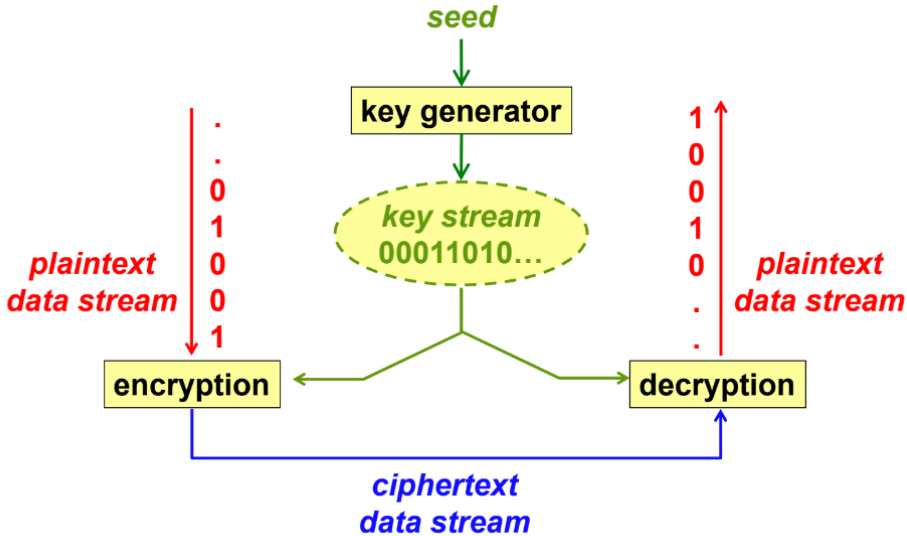
\includegraphics[width=\textwidth]{/home/lorenzo/Notes/Information System Security/images/Screenshot from 2024-12-28 11-20-36.png}
\end{minipage}
\noindent
\\
\\
The \textbf{K} is \textbf{randomly generated} and is used to XOR the \textbf{P} in order to obtain the \textbf{C}. This
makes stream algorithms really fast and unpredictable, which is good for security.
Decryption can be done \textbf{only} by using the \textbf{same K} \(\rightarrow \) if an attacker can delete part of the
\textbf{C}, decryption will be wrong since the \textbf{C}’s length is not the same as the \textbf{K}.
\noindent 
\begin{center}  
\begin{quotebox-grey}{Salsa20 and ChaCh20}

    \textbf{Salsa20} and \textbf{ChaCha20} are stream algorithms that use \textbf{128-256 bits K}. ChaCha20 is an improvement of Salsa20: it is \textbf{faster} on some architecture and has more \textbf{Diffusion Bits} (\(\rightarrow \) changing one input bits propagates the change t more output bits).
    \begin{itemize}
        \item Base Operation: 32 bits ARX(Add-Rotate-XOR).
        \item Base function: \(
        f(\text{Key}_{256}, \text{Nonce}_{64}, \text{Counter}_{64}) = 512 \text{-bit keystream block}
        \)
    \end{itemize}
    This allows \textbf{O(1)} decryption time for any random block. Salsa20 performs 20 random mixes of the \textbf{P}, while the \textbf{Salsa20/12} and \textbf{Salsa20/8} variants perform 12 and 8 respectively, making them faster but less secure. Meanwhile, ChaCha20 has been standardized and heavily adopted, especially in \textbf{IETF} Protocols. However, IETF uses a slightly modified version of ChaCha20
    that limits the maximum size of encryptable data to \textbf{256GB}. To overcome this limit we would need to use the original ChaCha20.
\end{quotebox-grey}
\end{center}

\section{Length of Secret Keys}
%	\vspace{-0.5cm}
The \textbf{K} should be adequate, meaning that if the encryption algorithm is well designed and the \textbf{K} is kept secret, then the \textbf{only} possible attack is a \textbf{Brute Force Attack} wich requires approximately: \[T=2^{Nbit}\]
(Where \(N^{Nbit}\) refers to the key lenght in bits). 
\\
\\
\\
\begin{minipage}{0.6\textwidth}
%	\vspace{-0.5cm}
\begin{itemize}
    \item \textbf{Symmetric Encryption Algorithms: K}s under 128 bits are \textbf{insecure}.
    \item \textbf{Asymmetric Encryption Algorithms: K}s under 2048 bits are \textbf{insecure}.
\end{itemize} 
\end{minipage} 
\hspace{0cm}
\begin{minipage}{0.4\textwidth}
    \centering
    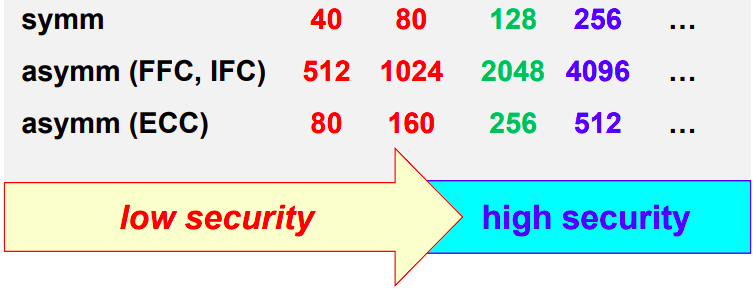
\includegraphics[width=0.8\textwidth]{/home/lorenzo/Notes/Information System Security/images/image copy 17.png}
\end{minipage}
\noindent
The area of low security increases with time, as computer become more powerful. Longer K means keeping data secret for longer, at the cost of an increase in time needed to encrypt data.
\newpage
\section{Asymmetric Cryptography}
\begin{minipage}{0.6\textwidth}
%	\vspace{-0.5cm}
Asymmetric Cryptography uses two different \textbf{K}:
\begin{itemize}
    \item \textbf{Private Key} (\textbf{SK})
    \item \textbf{Public Key} (\textbf{PK})
\end{itemize}
These keys are generated in such a way that \textbf{SK} \(\neq\) \textbf{PK}. The keys have \textbf{inverse functionality} \(\rightarrow \) data encrypted with one \textbf{K} can be decrypted \textbf{only} by the other \textbf{K}. This kind of cryptography has a \textbf{high computational load}, for that reason it is \textbf{only} used to transmit \textbf{K} used in Symmetric Cryptography and to create \textbf{digital signatures}.
\end{minipage} 
\hspace{0.3cm}
\begin{minipage}{0.4\textwidth}
    \centering
    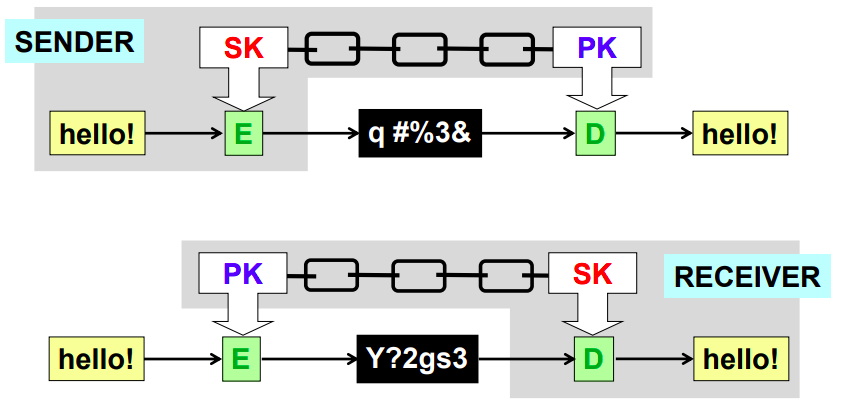
\includegraphics[width=\textwidth]{/home/lorenzo/Notes/Information System Security/images/image copy 18.png}
\end{minipage}

\subsection{Digital Signature}
\begin{minipage}{0.6\textwidth}
	\vspace{-0.3cm}
To perform a \textbf{digital signature} the author encrypts the message with its \textbf{SK}. The message can be then be decrypted by anyone who has access to the PK of the author. The message is \textbf{not} secret, but it is \textbf{signed by the author} (
    \(\rightarrow \) digital signature provides \textbf{data authN}) and \textbf{integrity}.
\end{minipage} 
\hspace{0.3cm}
\begin{minipage}{0.4\textwidth}
    \centering
    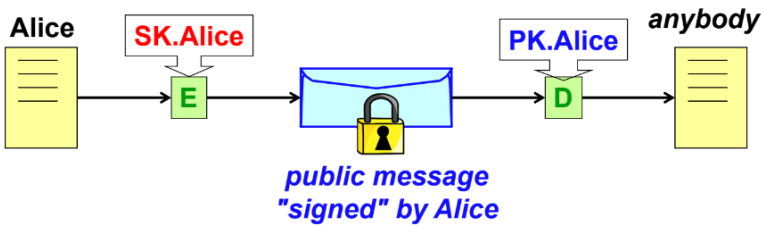
\includegraphics[width=\textwidth]{/home/lorenzo/Notes/Information System Security/images/Screenshot from 2024-12-28 15-25-58.png}
\end{minipage}
\subsection{Confidentiality without Shared Secrets}
\begin{minipage}{0.6\textwidth}
	\vspace{-0.6cm}
It is possible to generate a \textbf{secret message} for a particular \textbf{user X} just by encrypting it with
its PK. By doing so, we ensure that the message can \textbf{only} be decrypted by \textbf{X}, since \textbf{X} is the
\textbf{only one} who knows the \textbf{SK}. 
\end{minipage} 
\hspace{0.3cm}
\begin{minipage}{0.4\textwidth}
    \centering
    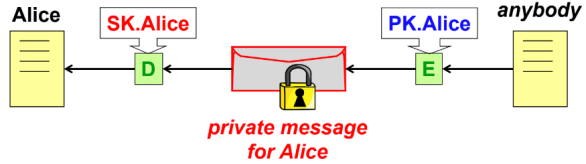
\includegraphics[width=\textwidth]{/home/lorenzo/Notes/Information System Security/images/Screenshot from 2024-12-28 15-28-47.png}
\end{minipage}
\vspace{-0.5cm}
\subsection{Secret Key Exchange}
\begin{minipage}{0.5\textwidth}
\vspace{-0.5cm}
Using asymmetric algorithms for secret key exchange enables confidentiality without
the need for shared secrets, and is often used to securely transmit a secret key for
symmetric encryption.
\end{minipage} 
\hspace{0.3cm}
\begin{minipage}{0.5\textwidth}
    \centering
    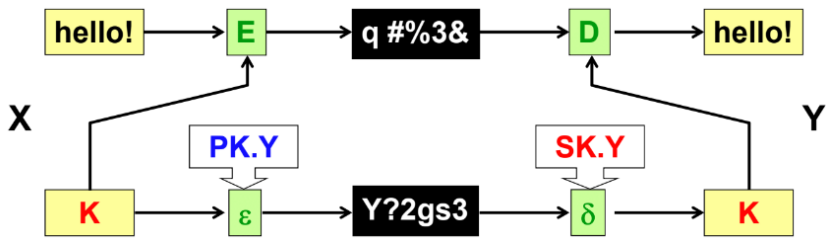
\includegraphics[width=0.8\textwidth]{/home/lorenzo/Notes/Information System Security/images/Screenshot from 2024-12-28 15-34-16.png}
\end{minipage}

\vspace{-0.2cm}
\noindent
\begin{center}
\begin{quotebox-yellow}{Diffie-Helmann Algorithm}
    The Diffie-Hellman (DH) algorithm is one of the first public-key algorithms invented and is primarily used for key agreement. The process is as follows:

    \begin{itemize}
        \item Alice (A) and Bob (B) agree on two public integers:
        \begin{itemize}
            \item \( p \): a large prime number
            \item \( g \): a primitive root modulo \( p \) (typically \( g = 2, 3, \) or \( 5 \))
        \end{itemize}
        \item The length of the DH key is determined by the number of bits in \( p \).
        \item Alice randomly chooses an integer \( x > 0 \) and computes:
        \(
        X = g^x \mod p
        \)
        \item Bob randomly chooses an integer \( y > 0 \) and computes:
        \(
        Y = g^y \mod p
        \)
        \item A and B exchange \( X \) and \( Y \).
        \item Alice computes the shared secret key:
        \(
        K_A = Y^x \mod p
        \)
        \item Bob computes the shared secret key:
        \(
        K_B = X^y \mod p
        \)
        \item It follows that:
        \(
        K_A = K_B = g^{xy} \mod (p)
        \)
    \end{itemize}
    Also this approach is not completely secure, since it can be
    attacked using the \textbf{Diffie-Hellman MITM attack}. The way in which the algorithm works and the attack is performed are explained by the following figures:
    \begin{figure}[H]
        \centering
        \vspace{-0.1cm}
        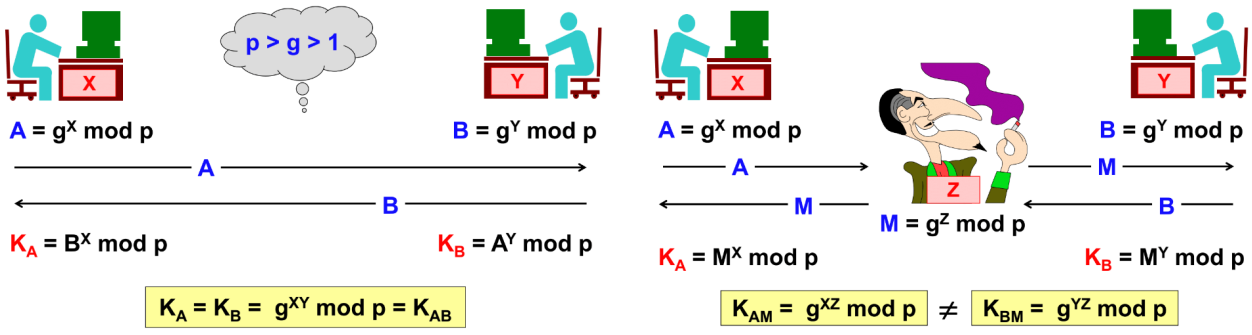
\includegraphics[width=0.6\textwidth]{/home/lorenzo/Notes/Information System Security/images/Screenshot from 2024-12-28 15-40-45.png}
    \end{figure}
\end{quotebox-yellow}
\end{center}

\subsection{Elliptic Curve Cryptography}

An \textbf{Elliptic Curve Cryptosystem (ECC)} executes operations on the surface of a 2D elliptic
curve, instead of using modular arithmetic. These problems are more complex than the modular
arithmetic ones, but at the same time they allow to use shorter keys (up to \(\frac{1}{10}\)). Most of the
algorithm we have seen (except RSA) have been revisited to adapt them to the elliptic curve:
\begin{itemize}
    \item \textbf{ECDSA} for Digital Signature;
    \item \textbf{ECDH} fro Key Agreement;
    \item \textbf{ECMQV} for AuthN Key Agreement;
    \item \textbf{ECIES} for Key Distribution;
\end{itemize}

\section{Digest for message integrity}
All the previous methods can guarantee (to a certain extent and for a certain time) that a message from a sender to the receiver \textbf{cannot} be understood by a third-party. However, it is still possible for an attacker to intercept the traffic from the 2 parties and \textbf{change} the encrypted message (Spoofing attack), even in an \textbf{unpredictable} way. Upon receiving the corrupted message, the receiver discard it and (probably) asks for retransmission, causing an(indirect) DoS attack.
\begin{center}
\begin{quotebox-red}{Beware}
Integrity is \textbf{not} about \textbf{preventing} modifications of data, it actually means that when data is received, the receiver can \textbf{verify} if the data has been modified or \textbf{not}.
\end{quotebox-red}
\end{center}
\noindent
\begin{minipage}{0.5\textwidth}
\vspace{-1.5cm}
To \textbf{guarantee integrity} the most common technique is to compute a \textbf{Digest}: fixed length summary of the whole message. Digests must be protected, as, conceptually, they are similar
to a checksum. But since checksum are easy to attack, Digests must to be calculated via a \textbf{Cryptographic Hash Function}.
\end{minipage} 
\hspace{0cm}
\begin{minipage}{0.5\textwidth}
    \centering
    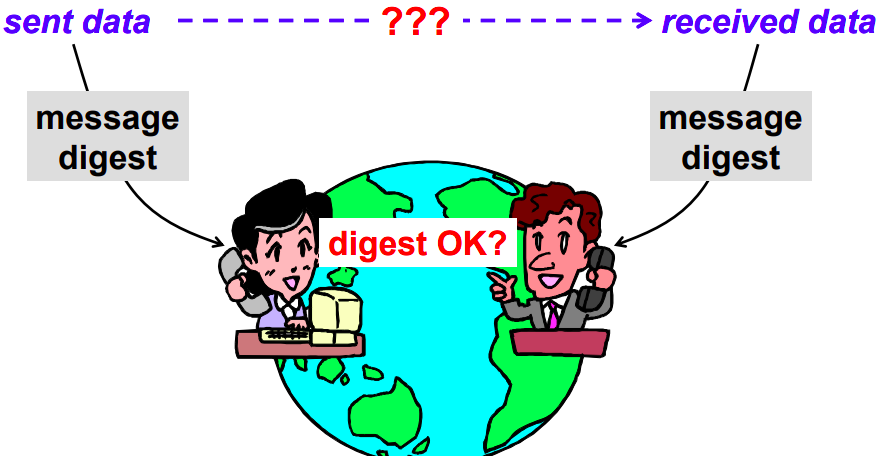
\includegraphics[width=0.8\textwidth]{/home/lorenzo/Notes/Information System Security/images/image copy 19.png}
\end{minipage}

\subsection{Hash Functions}
\textbf{Cryptographic Hash Functions} make Digests:
\begin{itemize}
    \item \textbf{Fast to compute}
    \item \textbf{Impossible or very difficult to invert}
\end{itemize}
Moreover, good Cryptographic Hash Functions should make it difficult to create  \textbf{Collisions}: collision happens when two different messages produce the same Digest.
Generally, Cryptographic Hash Functions work like this:
\\
\\
\begin{minipage}{0.6\textwidth}
	\vspace{-0.8cm}
\begin{enumerate}
    \item Split the message $M$ into $N$ blocks: $M_1, M_2, \dots, M_N$
    \item Iteratively applying a base function $f$ to each block.
    \[
    V_k = f(V_{k-1}, M_k) \quad \text{with} \quad V_0 = IV \quad \text{and} \quad h = V_N
    \]
\end{enumerate} 
\end{minipage} 
\hspace{0cm}
\begin{minipage}{0.4\textwidth}
    \centering
    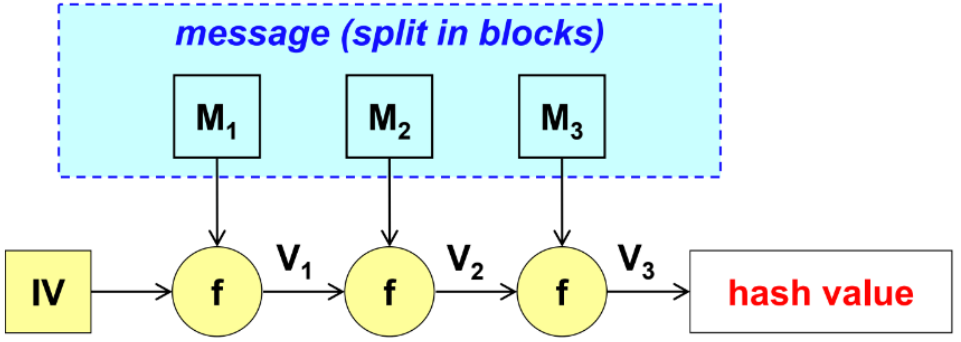
\includegraphics[width=\textwidth]{/home/lorenzo/Notes/Information System Security/images/Screenshot from 2024-12-28 16-13-17.png}
\end{minipage}

\begin{quotebox-grey}{Common Cryptographic Hash Functions}
    \begin{figure}[H]
        \centering
        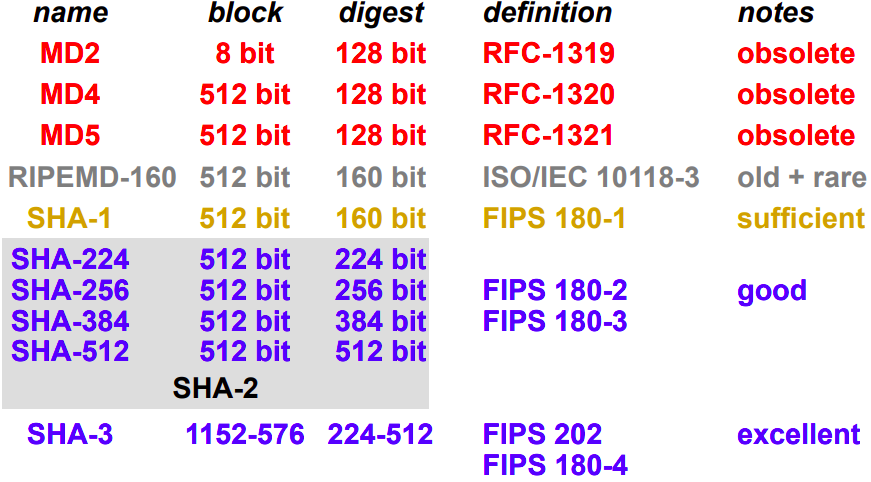
\includegraphics[width=0.5\textwidth]{/home/lorenzo/Notes/Information System Security/images/image copy 20.png}
    \end{figure}
\end{quotebox-grey}

\subsection{SHA-2 family}
Each algorithm in the \textbf{SHA-2 Family} has the same \textbf{block size (512 bits)}, but they have \textbf{increasingly higher Digest size}. The Digest size is important because a bigger Digest provoke less collisions (or aliasing).
If a Cryptographic Hash Function is \textbf{well designed} and generates a \(N_{bits}\) Digest, then the \textbf{probability of aliasing} is: \[P_A \propto \frac{1}{2^N}\]
\vspace{-0.3cm}
\begin{center}
    \begin{quotebox-red}{Birthday Paradox}
        The \textbf{Birthday Paradox} is a statistical consideration that warns us of the risks of making Digests too big: a \(N_{bits}\) Digest is \textbf{insecure} when more than \(2^{\frac{N}{2}}\) digests are generated. This is because the probability to have a collision is \textbf{PA \(\thicksim\) 50\%}.
    \end{quotebox-red}
\end{center}
\textcolor{red}{\textbf{N.B.}} A cryptosystem is \textbf{balanced} when the Encryption algorithm and Digest function have the same resistance. For example, SHA-256 and SHA-512 have been designed for AES-128 and AES-256 respectively.
\subsection{SHA-3 family}
SHA-3 is based on the \textbf{Keccak} algorithm, it uses an elegant design that is easy to analyse and performs very well on many different computing devices.
\begin{figure}[H]
    \centering
    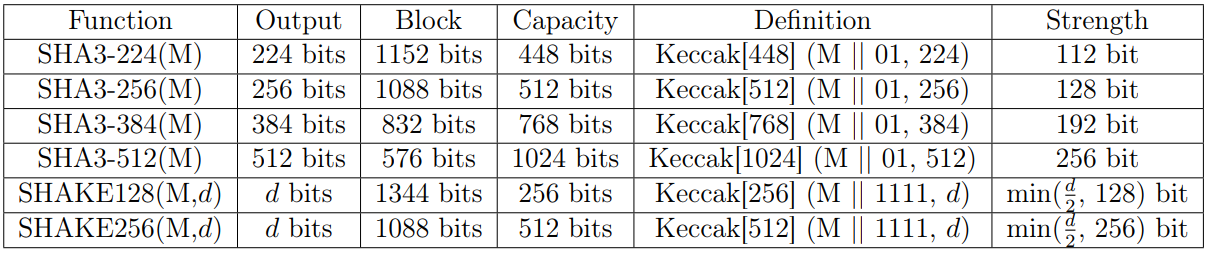
\includegraphics[width=0.7\textwidth]{/home/lorenzo/Notes/Information System Security/images/Screenshot from 2024-12-28 17-37-14.png}
\end{figure}
\section{KDF (Key Derivation Function)}
KDFs are \textbf{Cryptographic Hash Functions} used to create a random \textbf{K}:
\[
K = \text{KDF}(P, S, I)
\]
Where:
\begin{itemize}
    \item \textbf{\( P \) is the password} or passphrase.
    \item \textbf{\( S \) is the salt}, which makes the key \( K \) harder to guess given \( P \).
    \item \textbf{\( I \) is the number of iterations}, used to slow down the computation and increase security.
\end{itemize}
\noindent
\begin{customquote}
The main KDF is \textbf{PBKDF2}:
\[
\text{DK} = \text{PBKDF2}(\text{PRF}, \text{P}, \text{S}, I, \text{dkLen})
\]
Where \textbf{P}, \textbf{S} and \textbf{I} are the same as above, while:
\begin{itemize}
    \item \textbf{PRF}: is a \textbf{Pseudo-Random Function} that outputs a value of lenght \textbf{hLen}.
    \item \textbf{dkLen}: is the \textbf{Desired Lenght of the DK}.
\end{itemize}
The derived key, \( DK \), is generated by concatenating subkeys \( T_1, T_2, \dots, T_{dkLen/hLen} \), where each \( |T_i| = hLen \).
\end{customquote}
\noindent{\color{gray!50}\rule{\textwidth}{0.5pt}}
\section{MIC, MAC \& MID}
In the telecommunication and networking environment, the \textbf{MIC (Message Integrity Code)} is the code that is added to the message to guarantee integrity. Meanwhile, in the application
field, the same code is named MAC (Message Authentication Field), since, if the message
has not been modified \(\rightarrow \) data authN.\\
Since the MIC/MAC code is an addition to the original message, a \textbf{unique MID} (\textbf{Message IDentifier}) is also concatenated with the message, in order to avoid Replay attacks.

\section{Digest Protection}
In the simple case in which a Digest is used to verify that a file on disk has not been changed, a good approach could be to store the digest in a \textbf{different and secure place}. But when the data is being \textbf{transmitted}, Digests \textbf{cannot} be exchanged OOB \(\rightarrow \) Digests \textbf{must be intrinsically secure}. To achieve this, there are two main techniques:
\begin{itemize}
    \item \textbf{AuthN by means of Keyed Digest}
    \item \textbf{Authenticated Encryption}
\end{itemize}

\subsection{AuthN by means of Keyed Digest}
The Digest \textbf{d} is sent along with the message \textbf{M}, but it is calculated using \textbf{both} the \textbf{M} and the
\textbf{K}, which is shared \textbf{only} between sender and receiver (symmetric key).
\\
\\
\begin{minipage}{0.5\textwidth}
\vspace{-1cm}
The following operations are perfomed:
\begin{itemize}
    \item \textbf{Sender}: \(d = \text{digest}(K, M)\).
    \item \textbf{Transmission}: \(M || d\).
    \item \textbf{Receiver}: \(d' = \text{digest}(K, M)\).
    \item \textbf{Verification}: If \(d == d'\), the message is authenticated, otherwise an alarm is raised.
\end{itemize}

\end{minipage} 
\hspace{0.3cm}
\begin{minipage}{0.5\textwidth}
    \centering
    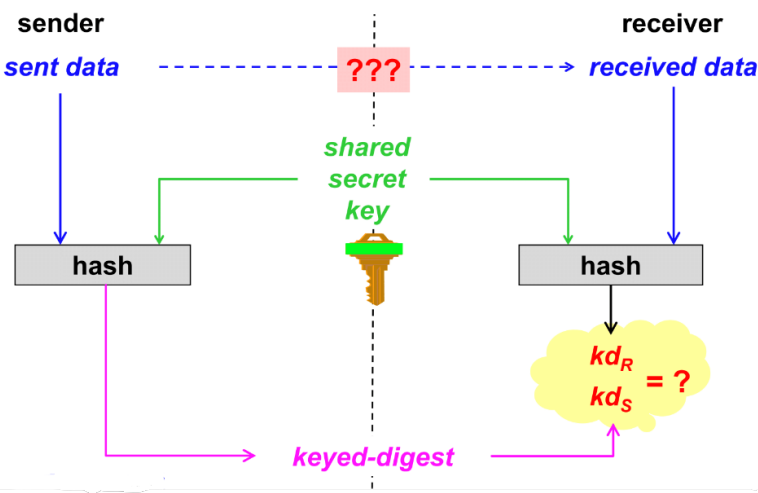
\includegraphics[width=0.6\textwidth]{/home/lorenzo/Notes/Information System Security/images/Screenshot from 2024-12-28 17-18-08.png}
\end{minipage}

\noindent
This technique also guarantees \textbf{data authN}, since \textbf{only} who knows the \textbf{K} can compare the receive digest with the one calculated from the received data (\(\rightarrow \) the Keyed Digest is the fastest way to guarantee \textbf{integrity} and \textbf{data authN}).
\vspace{-0.5cm}
\begin{center}
    \begin{quotebox-red}{}
        However, it does \textbf{not} provide \textbf{non-repudiation}, since it is \textbf{not} possible to determine which
        party created the data, because both have the means (data and \textbf{K}) to create the Keyed Digest.
    \end{quotebox-red}   
\end{center}
\begin{itemize}
    \item \textbf{HMAC}: is the \textbf{best way} to compute a \textbf{secure MAC} starting from a hash function \textbf{H}.
    \textbf{H} must have a block of size \textbf{B} bytes, an output of \textbf{L} bytes, where \(B > L\).\\ Moreover, in order to work with HMAC we need:
    \begin{itemize}
        \item \textbf{ipad}: \(0x36\) repeated \(B\) times.
        \item \textbf{opad}: \(0x5C\) repeated \(B\) times.
        \item A \textbf{K} bigger or equal to \textbf{L} (\( |K| > L \)). \textbf{Never} use a \textbf{K} smaller than \textbf{L}! (e.g using SHA-1 with HMAC means that \textbf{K must} be of \textbf{at least 160 bits}):
        \begin{itemize}
            \item if \(|K| > B\) \(\rightarrow \) \(K'=H(K)\).
            \item else \(\rightarrow \) \(K'=K\).
            \item if \(|K'|>B\) \(\rightarrow \) \(K'\) is 0-padded up to \textbf{B} bytes; 
        \end{itemize}
    \end{itemize}
    \[
        \text{hmac-H} = H\left( K' \oplus \text{opad} || H(K' \oplus \text{ipad} || \text{data}) \right)
        \]
    \item \textbf{CBC-MAC}: is another way to compute a digest \textbf{without} using a hash function, but just by using a Symmetric Encryption Block Algorithm, which is applied in CBC mode and using a \textbf{null IV}. Of the whole algorithm's output, \textbf{only} the \textbf{last (encrypted) block} is used as the \textbf{MAC}.
    \\ 
    \begin{customquote}
    \vspace{-0.4cm}
    \subsubsection{Process}
    \begin{itemize}
        \item The message \(M\) is split into \(N\) blocks \(M_1, M_2, \dots, M_N\).
        \item The MAC is computed iteratively: \(V_0 = 0\) and for each block \(k\), compute:
        \[
        V_k = \text{enc}(K, M_k \oplus V_{k-1})
        \]
        \item The final MAC is the last encrypted block \(V_N\).
    \end{itemize}
    \end{customquote}
    CBC-MAC does \textbf{not} guarantee \textbf{confidentiality} because the IV is fixed, but it guarantees \textbf{integrity} thanks to CBC: if the message is modified in any point, the last (encrypted) block \textbf{will} be different.\\
    \textcolor{red}{\textbf{N.B.}} CBC-MAC is secure \textbf{only} for fixed-lenght message \(\rightarrow \) attacks that change the length of the message can be successful.
\end{itemize}

\section{Integrity \& Confidentiality Combinations}
\textbf{Integrity} and \textbf{confidentiality} can both be achieved with the combined use of two algorithms
and with \textbf{two distinct K}s:
\begin{itemize}
    \item Symmetric Encryption with \(K_1\) is used to gain \textbf{confidentiality}.
    \item AuthN by means of Keyed Digest with \(K_2\) is used for \textbf{integrity}.
\end{itemize}
There are various ways to combine these two algorithms:
\begin{itemize}
    \item \textbf{A\&E (Authenticate \& Encrypt)}: Encrypt the message and then authenticate it using a MAC. Insecure unless performed as a single step (used by SSH).
    \[enc(K_1.P)\ ||\ mac(K_2,P)\]
    \item \textbf{AtE (Authenticate then Encrypt)}: compute the MAC on the plaintext and then encrypt both the message and MAC. Secure if used with CBC or stream encryption (used by SSL and TLS). The \textbf{Ate} is still vulnerable to DoS attacks.
    \[enc(K_1,P\ ||\ mac(K_2,P))\]
    \vspace{-0.6cm}
    \item \textbf{EtA (Encrypt-then-Authenticate)}: Encrypt the message, then compute the MAC on the ciphertext. This is the most secure method (used by IPsec). With \textbf{AtE} solution is possible to avoid DoS attacks since the MAC can be calculated using \textbf{C} (fast operation) \textbf{without} the need to decrypt it (slow operation).
    \[C=enc(K_1,P)\rightarrow C\ ||\ mac(K_2,C)\]
\end{itemize}

\section{AE (Authenticated Encryption)}

The \textbf{AE} concept uses a \textbf{single operation} that, once performed, guarantees: \textbf{payload confidentiality}, \textbf{data authN} and \textbf{integrity}. This is achieved by using just a \textbf{single K} and a
\textbf{single algorithm} \(\rightarrow \)  \textbf{better speed} and less likelihood of errors due to the combination of different functions. 
\begin{figure}[H]
    \centering
    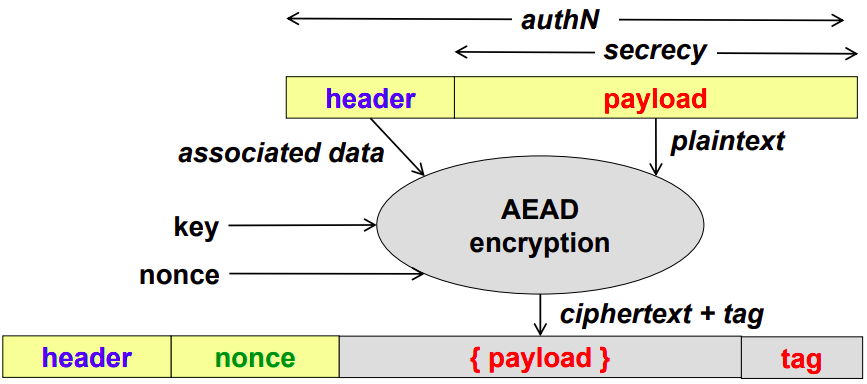
\includegraphics[width=0.5\textwidth]{/home/lorenzo/Notes/Information System Security/images/image copy 21.png}
\end{figure}
\begin{quotebox-red}{Beware}
    AE does \textbf{not} provide \textbf{non-repudiation} because both peers share the same key.
\end{quotebox-red}
\vspace{0.1cm}
\noindent
AE can work in 6 standard modes:
\begin{itemize}
    \item \textbf{OCB 2.0} (Offset Codebook Mode): the fastest one, on-line single-pass AEAD.
    \item \textbf{AESKW} (AES Key Wrap).
    \item \textbf{CCM} (CTR mode with CBC-MAC): the slowest one, off-line double-pass (half as fast as
    single-pass).
    \item \textbf{EAX} (EtA then (X)translate): very good for constrained systems, on-line double-pass
    AEAD.
    \item \textbf{Encrypt then MAC}
    \item \textbf{GCM} (Galois/Counter Mode): the most popular one, on-line single-pass AEAD, it is
    also parallelizable.
\end{itemize}
A \textbf{lightweight environment} solution to all of this modes is \textbf{ASCON}.
\vspace{0.2cm}
\begin{customquote}
\vspace{-0.4cm}
\subsubsection{IGE (Infinite Grable Extension)}
\begin{minipage}{0.5\textwidth}
	\vspace{-0.5cm}
IGE is an \textbf{AE algorithm} that works like
CBC, but with one addition that makes
any \textbf{modification} of any block \textbf{propagate
to every block after that one}.\\
This is important, because it means that
by having the last block with fixed content
\(\rightarrow \) in the decryption phase \textbf{integrity is verified only if} the last block has the excepted content. 
\end{minipage} 
\hspace{0cm}
\begin{minipage}{0.4\textwidth}
    \centering
    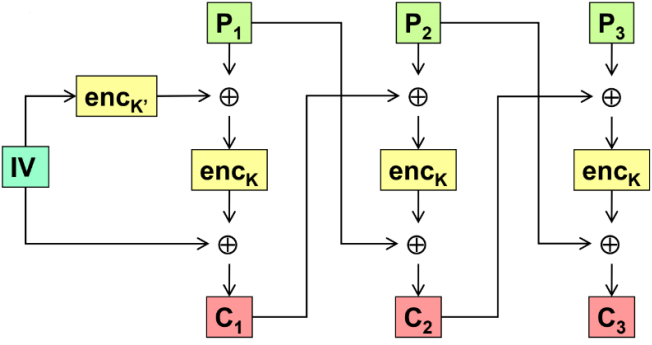
\includegraphics[width=0.7\textwidth]{/home/lorenzo/Notes/Information System Security/images/Screenshot from 2024-12-29 12-20-11.png}
\end{minipage}

\end{customquote}

\section{Digital Signature}